\documentclass[mathserif]{beamer} 
\usefonttheme{professionalfonts}
\usefonttheme{serif}
\usetheme{YYY}
\usepackage[orientation=landscape,size=custom,width=118.9,height=84.1,scale=1.05,debug]{beamerposter}
\usepackage[absolute,overlay]{textpos} 
\usepackage{color}
\usepackage{graphicx}
\usepackage{caption} 
\usepackage{multicol}
\setlength{\TPHorizModule}{1cm}
\setlength{\TPVertModule}{1cm}

\title{\quad\quad{XXX}}
\date{}

\begin{document}
\begin{frame}{~} 
\begin{columns}[t]

\column{.45\textwidth}
\begin{block}{Research Questions}
\begin{itemize}
\item 
\end{itemize}
\end{block}

\begin{block}{Theory}
\begin{itemize}
	\item
\end{itemize}	
\end{block}	

\begin{block}{Hypotheses}
\begin{itemize}
	\item 
\end{itemize}	
\end{block}	

\begin{block}{Data and Method}
\begin{itemize}
\item 
\end{itemize} 
\end{block}

\begin{block}{Regression Table}
	\begin{table}[h!]\centering
		\begin{tabular}{l l l l}
			\hline\hline\noalign{\smallskip}
			&\multicolumn{1}{c}{Model 1}&\multicolumn{1}{c}{Model 2}&\multicolumn{1}{c}{Model 3}\\
			\hline
			Secessionist        &      -0.482***         &      -0.437**         &          -0.338*           \\
			&     (0.140)         &     (0.139)         &         (0.170)            \\
			[1em]
			Territorial Control &                     &       0.352**         &       0.427**          \\
			&                     &     (0.128)         &        (0.147)            \\
			[1em]
			Secessionist $\times$ Territorial Control&                     &                     &      -0.304         \\
			&                     &                     &     (0.298)         \\
			[1em]
			Constant            &       4.882***&       4.734***  &       4.702***         \\
			&     (0.073)         &     (0.091)         &     (0.096)         \\
			\hline
			Observations        &         334         &         334         &         334         \\
			\(R^{2}\)           &       0.035         &       0.056         &       0.059         \\
			\hline\hline
			\multicolumn{4}{l}{\footnotesize Standard errors in parentheses. {*} \(p<0.05\), {**} \(p<0.01\), {***} \(p<0.001\).} \\
			\noalign{\smallskip}\hline
		\end{tabular}
	\end{table}
\end{block}

\begin{block}{Results}
\begin{itemize}
	\item XXX
	\begin{itemize}
	    \item XXX 
	\end{itemize}	
\end{itemize}	
\end{block}	

\column{.45\textwidth}
\begin{block}{Plots}
\begin{multicols}{2}
		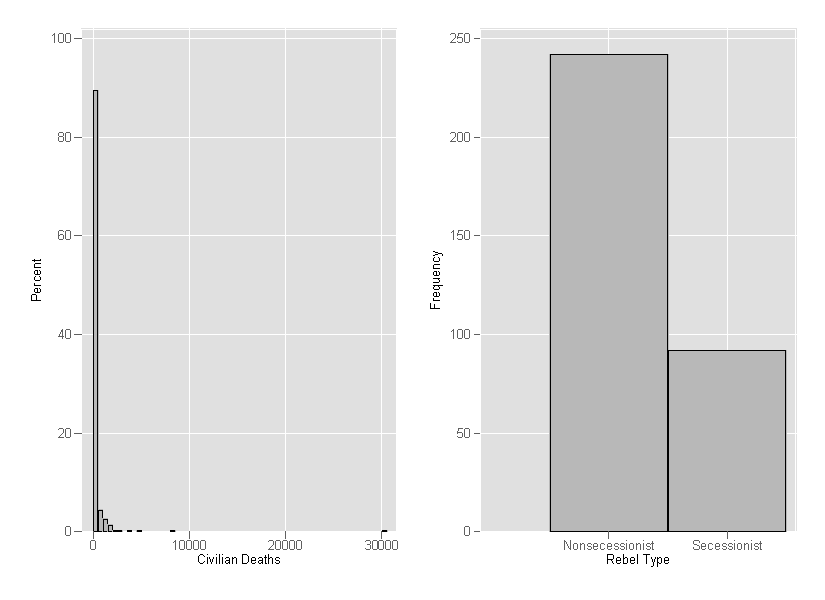
\includegraphics[width=1\linewidth, height=1\linewidth]{DVIVhist.pdf}
		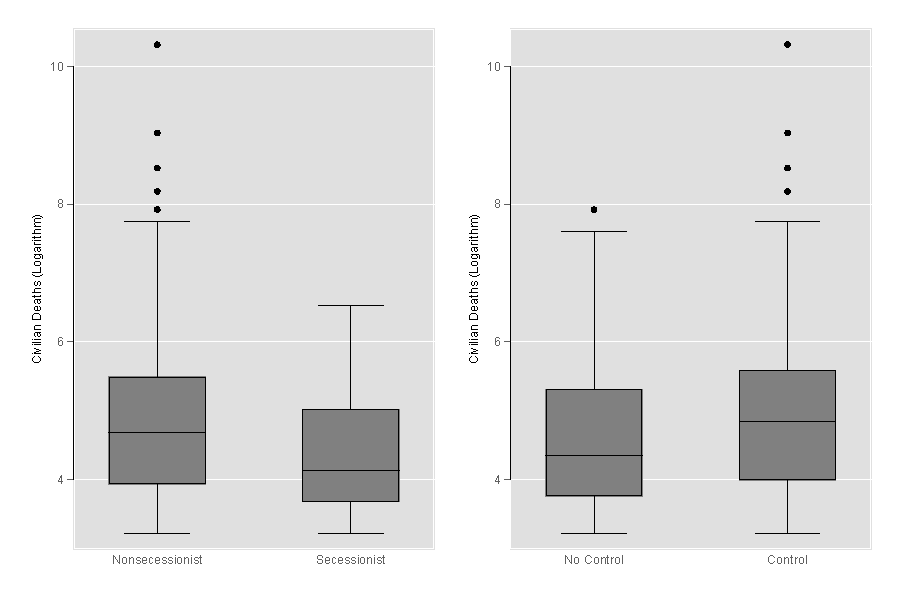
\includegraphics[width=1\linewidth, height=1\linewidth]{DVIVTERRbox.pdf}
\end{multicols}
\end{block}

\begin{block}{Conclusion}
\begin{itemize}
\item
\end{itemize}
\end{block}

\end{columns}
\end{frame}
\end{document}
